
Previously, we discussed the dynamics of \eqref{eq:magnetichamiltonian2} from the perspective of perturbation theory. Now, we attempt to extract some meaningful symbolic dynamics. We specify \textit{meaningful} dynamics because we fail to do so via the standard approach: finding a markov partition and a conjugation to the shift map, instead we consider a reasonable map into a symbol space and judge the dynamics via the Lempel-Ziv complexity measure. What we find is two complementary methods to characterize the dynamics.

\subsection{Constructing a Poincar\'e section}

To simplify the notation, we consider motion in the torus $\mathbb T=[0,1]^2$, this way we need only refer to one disk $S= \{x\in \mathbb T : \|x-1/2\|\le R\}$. We recall the trajectories have two modes: linear outside the magnetic disk $S$, and along circular arcs within the disk. Consider two subsets $\Sin,\Sout\subset \mathbb T\times\mathbb R^2$ of phase space defined by:
\begin{align}
\label{def:poincaresectionIN}
\Sin &= \bigcup_{x\in\partial S} \{x\} \times \{v\in\mathbb R^2 : v\cdot (x-1/2) < 0\},\\
\label{def:poincaresectionOUT}
\Sout &= \bigcup_{x\in\partial S} \{x\} \times \{v\in\mathbb R^2 : v\cdot (x-1/2) > 0\},
\end{align}
so $\Sin$ is the part of phase space that lies on the boundary $\partial S$ and has velocity vector pointing into $S$, while $\Sout$ points outward. Notice that we exclude velocities that are tangential to $\partial S$. We show now that both $\Sin$ and $\Sout$ are poincare sections of the full system.

\begin{lemma}
The flow of \eqref{eq:magnetichamiltonian2} induces a well-defined map $P_\text{io}:\Sin\to\Sout$.
\end{lemma}
\begin{proof}
Let $(x,v)\in \Sin$, under the flow of \eqref{eq:magnetichamiltonian2} we know the Larmor circle $C$ with initial conditions $(x,v)$ intersects $\partial S$ in $x$ and that at $x$ the circles are not tangential. Two circles intersecting at a point non-tangentially must intersect at a second point, so there exists $x\neq y\in\partial S\cap C$. By the flow of \eqref{eq:magnetichamiltonian2} there must also exist a velocity $w\in\mathbb R^2$ such that $w\cdot(x-1/2)>0$, that is $(y,w)\in\Sout$. Hence we have $P_\text{io}(x,v) = (y,w)$. 
\end{proof}

We can say more, there exists a line $\ell$ through the center $a$ of the Larmor circle $C$ and the center $(1/2,1/2)$ of $\partial S$. The two circles are symmetric with respect to the reflection $T$ with respect to $\ell$. This means $Tx=y$, and $Tv = -w$. The following statement is more interesting.

\begin{lemma}
The flow of \eqref{eq:magnetichamiltonian2} induces a well-defined map $P_\text{oi}:\Sout\to\Sin$.
\end{lemma}
\begin{proof}
Let $(x,v)\in\Sout$, then under the flow of \eqref{eq:magnetichamiltonian2} we see linear motion. Ignoring the presence of $S$, we see that depending on $v$, the trajectory is either periodic or is dense in $\mathbb T$.

Focusing on the first case, in finite time we return to the point $x$. Since the trajectory is a line $\ell$ interesecting $\partial S$ transversally, there must be another point of intersection $x\neq y\in\partial S\cap\ell$. The velocity at $y$ must also be $v$, so due to the geometry of a circle, $(y,v)\in\Sin$. For the second case, we can pick $\varepsilon>0$ such that all points in $U=(\partial S\cap B_\varepsilon(x))\times\{v\}\subset \Sout$ are transversal to $\partial S$. Let $(y,v)\in U$, since the flow is dense for the velocity $v$, ignoring $S$, we know that in finite time the point $(x,v)$ comes to $(y,v)$. The rest of this case follows the same way as previously. 

In either case, the $(y,v)$ we find is not necessarily the first time we enter $\Sin$ but since the number of such points is countable, we can pick the first one $(y_0,v)$, hence, $P_\text{oi}(x,v) = (y_0,v)$ is a well-defined map.
\end{proof}

Now, we can finalize the Poincar\'e map.

\begin{proposition}
The sets $\Sin$ and $\Sout$ are Poincar\'e sections with Poincar\'e maps $P_\text{in} = P_\text{oi}\circ P_\text{io}$ and $P_\text{out}= P_\text{io}\circ P_\text{oi}$, respectively.
\end{proposition}

Notice that the reasoning is independent of the radius of $S$, nor does it depend on the exact position of $S$. Pulling back to the plane with an infinite number of disks, we can then generalize the setup. Consider a fundamental finite set $A$ of disks where each disk in $A$ can have a different magnetic strength and radius and the disks need not be regularly placed. The above result holds for configurations of disks which can be decomposed as a tiling of such a set $A$.

In \cite{Knauf_2017} a similar result is proved for a configuration of finitely many bumps. In that case a different method was used that did not rely on an infinite number of bumps, in ours the reasoning was simplified due to this.

\subsection{Some simple periodic trajectories}

With the Poincar\'e map we can already study the stability of periodic trajectories of the system. We provide some simple examples in this section, and prove the (in)-stability of some. The examples were found by trial and error, and with some imagination. We will detect more complicated periodicity in the section where we introduce the Lempel-Ziv complexity. We present some periodic orbits in FIG, the parameters and initial conditions can be found in the TABLE



The code written in \texttt{Python} utilizes the symbolic algebra system \texttt{Sympy} to define functions, compute derivatives, compose functions, and compute eigenvalues of a Jacobian symbolically. That way we avoid a considerable amount of computation by hand but still retain a high degree of precision when computing numerical values. For long enough periodic orbits, the computation time using symbolic algebra becomes unreasonable, so we require a different way to analyse stability. A common alternative is to compute Lyapunov exponents of the original system or of the Poincar\'e map. However, these approaches are prone to numerical instability and require significant preparation beforehand. We would like to analyze stability from the trajectory directly, and we attempt this via symbolic dynamics in the next section.


\color{red}
With $B_r(q)\subset \mathbb R^2$ denote the closed ball of radius $r>0$ centered at $q\in\mathbb R^2$. Pick $S=\cup_{N\in\mathbb Z^2}B_{1/3}(N-1/2)$, that is, $S$ is the union of closed balls of radius $1/3$ centered at points of the form $(n-1/2,m-1/2)$ for $n,m\in\mathbb Z$.

The choice of radius $r=1/3$ is arbitrary, we fix it for convenience. Furthermore, we notice the speed of the particle is constant, since $\|X'(0)\|=Rb$, so again for simplicity we fix $\|X'(0)\|=1$. This also fixes the Larmor radius $R=1/b$. A different choice of $r\in (0,1/2)$ and $\|X'(0)\|\in(0,\infty)$ clearly gives rise to different dynamics, however we make the assumption that the dynamics will not differ \textit{qualitatively}, i.e., in any case we expect to find periodic orbits, chaotic behavior, and the methods we use for studying these are still valid.

Hence, we study the influence of varying the parameter $b>0$ on the above defined system. What we see is four ranges of behavior:
\begin{enumerate}
\item For values $b\approx0$ we can approximate the dynamics as a perturbation of a system with no magnetic field at all,
\item For a range of ``small'' values of $b$, the dynamics are similar to that of a uniform field in $\mathbb R^2$,
\item there is an intermediate range where both stable and unstable periodic dynamics occur
\item there exists a value $b_t$, such that all values $b>b_t$ give rise to unstable dynamics.
\end{enumerate}

We can use this to already find some simple periodic orbits. We describe one such orbit now.

Let $\delta\in(0,1/3)$ and consider the initial condition $(x,p) = (0,1/2+delta,1,0)$, the trajectory can be seen in \cref{subfig:periodicorbit1}. We can compute that for the choice $b=1/\delta$, the trajectory will be a periodic orbit.

Already, we see that periodic orbits exist for arbitrarily large $b$. It can be shown using Poincar\'e sections that this family of periodic orbits is unstable.

Another family of periodic orbits are given for $\delta\in(-1/\sqrt{18},1/3)$, where the initial condition is $(x,p)=(0,1/2+\delta,1,0)$ and $b = 1/(\delta+\sqrt{1/9-\delta^2})$

Another family of periodic orbits are given for $\delta\in(1/\sqrt{18},1/3)$, where the initial condition is $(x,p)=(0,1/2+\delta,1,0)$ and $b = 1/(\delta-\sqrt{1/9-\delta^2})$

Lastly, we have a more complicated periodic orbit that forms an octagon for 


\begin{figure}[!th]
\centering
\begin{subfigure}{0.49\textwidth}
\centering
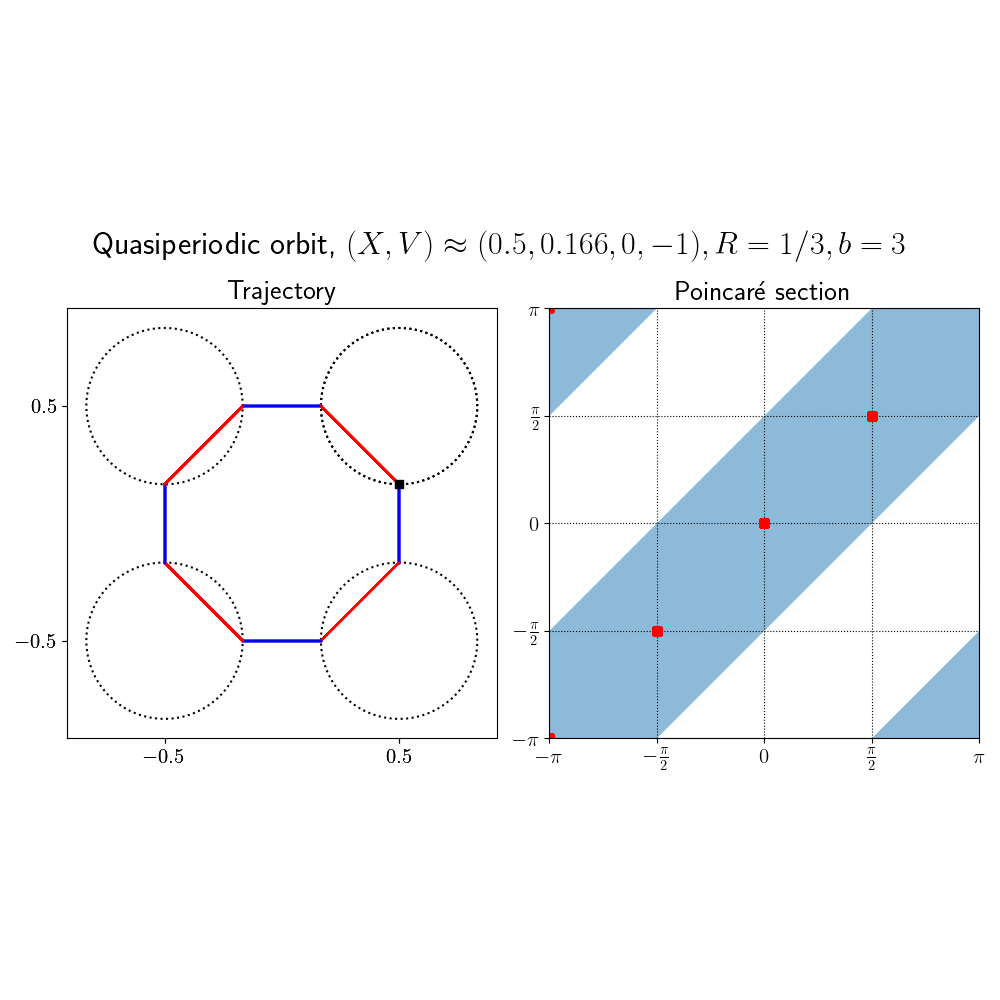
\includegraphics[width=\textwidth, trim={0 5.5cm 0 5.5cm}, clip]{fig5.png}
\caption{say smth albert}
\label{subfig:periodicorbit1}
\end{subfigure}
%
\begin{subfigure}{0.49\textwidth}
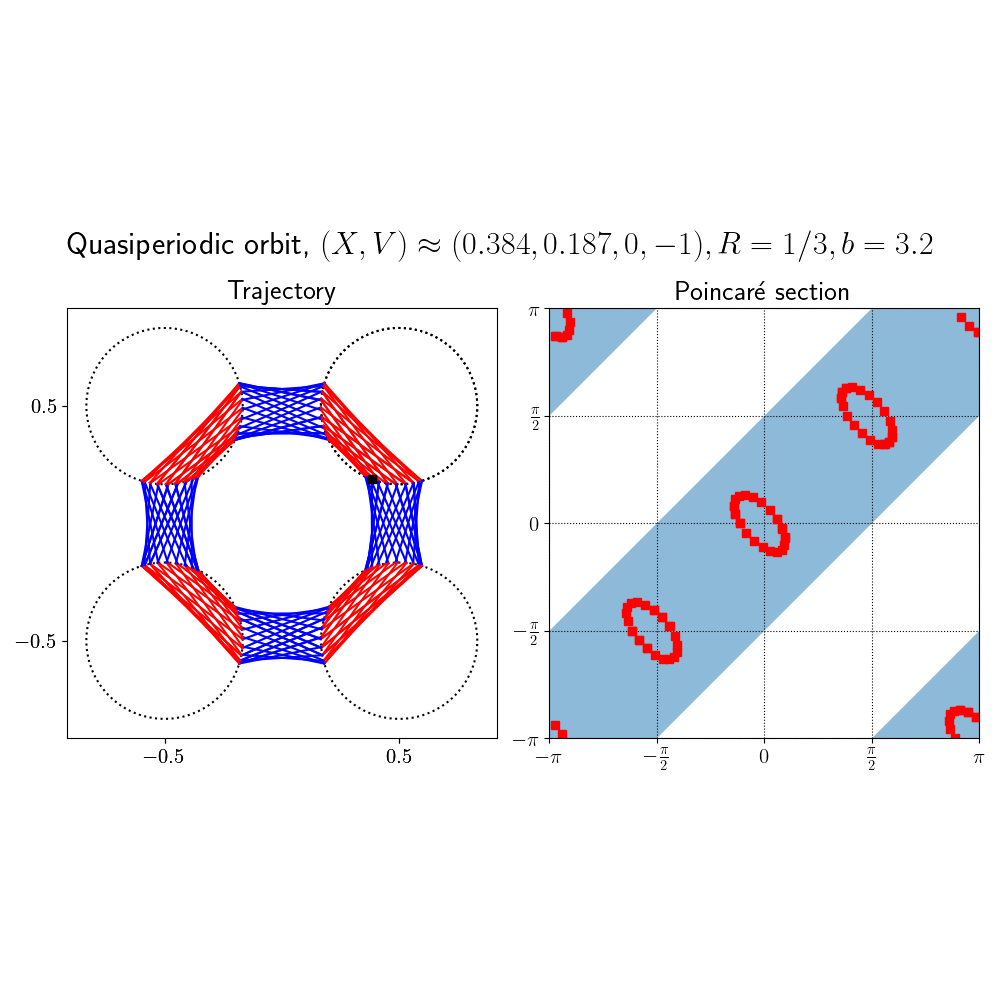
\includegraphics[width=\textwidth, trim={0 5.5cm 0 5.5cm}, clip]{fig4.png}
\caption{say smth albert}
\label{subfig:periodicorbit2}
\end{subfigure}
%
\begin{subfigure}{0.49\textwidth}
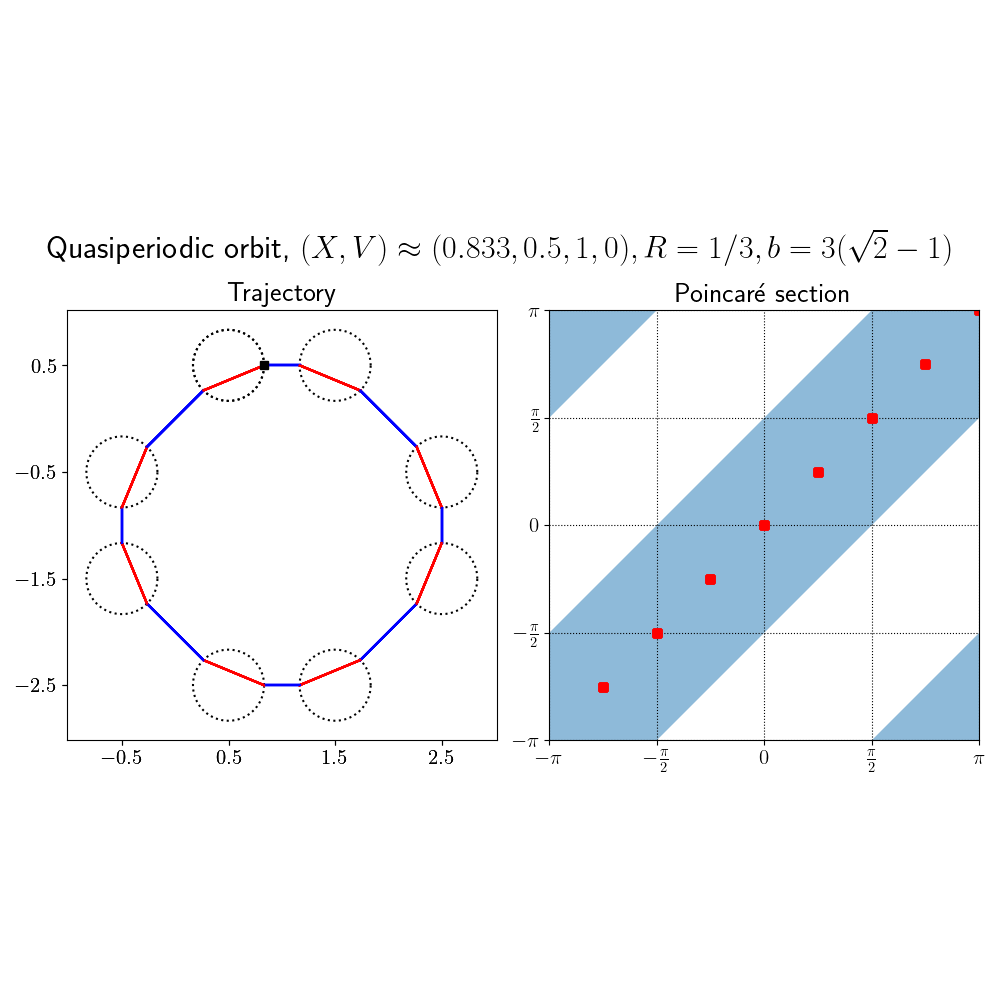
\includegraphics[width=\textwidth, trim={0 5.5cm 0 5.5cm}, clip]{fig6.png}
\caption{a.}
\label{subfig:periodicorbit3}
\end{subfigure}
%
\begin{subfigure}{0.49\textwidth}
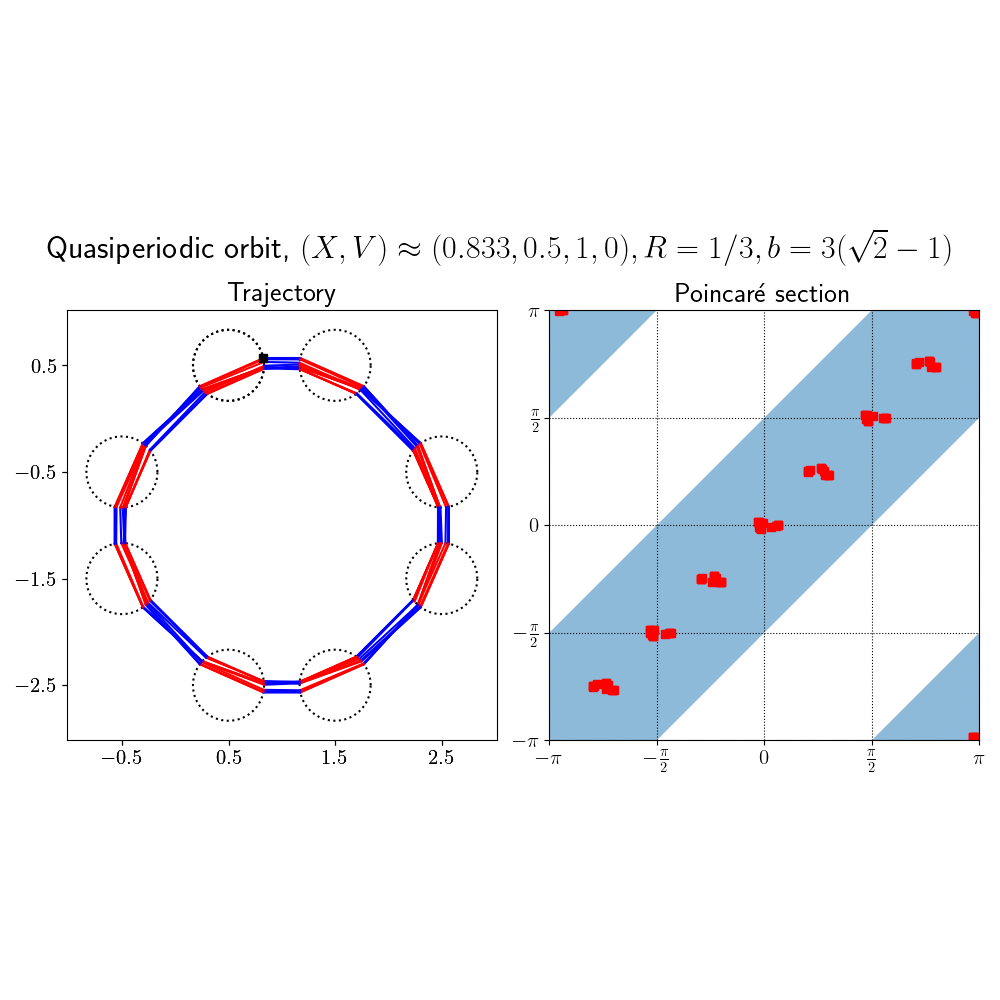
\includegraphics[width=\textwidth, trim={0 5.5cm 0 5.5cm}, clip]{fig7.png}
\caption{.}
\label{subfig:periodicorbit4}
\end{subfigure}
\caption{Examples of periodic, quasiperiodic, and aperiodic trajectories for varying choices of parameters.}
\label{fig:periodicorbits}
\end{figure}

\color{black}